% Pictures of input devices?
\section{System Design \& Implementation}\label{sec:design}

Driven by the requirements of the experiment design, we created a testing
platform based on a standard desktop computer, various input devices, a USB
camera, and a 3D stereoscopic monitor.  These components are described in
detail below.

\subsection{Input Devices}
The goal with our input device selection and interface design was to isolate
the characteristics of the input method to be applicable to many types of
device.  Thus our conclusions using the Leap Motion should be transferable to
any in-air, free-hand input mechanism, our conclusions with the mouse should
be applicable to the trackball, and so on.

While our original inspiration was to compare standard mouse and keyboard
interfaces with 1-to-1 free space interfaces, we recognized that other devices
have been designed and tested for 3D tasks. These include 3D-joystick analogs
such as the SpaceNavigator \cite{mattheiss2011navigating}; 6-DOF tracked
wand-based systems that function in relative space rather than absolute space,
such as the Wiimote or Razer Hydra; and paired input devices to be used by both
hands simultaneously such as the DepthSlider \cite{study1}. To limit the length
of our experiment we elected to investigate only the wand-based 3D relative
input devices in addition to the mouse interface and the aligned free-space
interface.

For each input device, we also considered the particular interactions
experiment participants would perform. In particular, we decided to evaluate
performance on a 3D selection task with only three degrees of freedom (see
Section~\ref{sec:experiment}) rather than a docking task that involved
position and orientation, which would require six degrees of freedom. We also
did not allow users to control the viewpoint beyond head tracking. These
decisions were made to preserve the ``purity'' of our input device evaluation,
since while intuitive mappings from input device movement to 3D position are
fairly obvious and are arguably implied by the device design, camera control
movements and arbitrary rotational movements are much less so.

For our task, each input device needs to two things: {\it point}, specifying a
point in the 3D space, and {\it click}, indicating acceptance of the current
point. We refer to {\it relative} and {\it absolute} input devices, where
absolute input devices have a direct 1-to-1 spatial relationship with the
virtual space (i.e. a rotation, uniform scaling, and translation maps virtual
space to real world space) while relative input devices preserve directions
but may map magnitudes of motions non-linearly. Standard mice and touchpads
are relative, not absolute, since faster movements across the same physical
distance map to larger mouse pointer movements. A device such as a trackball
or joystick is neither relative nor absolute, since they don't move spatially.

\subsubsection{Mouse and Keyboard (2D Relative Interface)}
Our mouse and keyboard interface mimics the input mechanisms used in standard
3D modelling software. To achieve precise arbitrary spatial positioning, the
standard interaction involves several orthogonal projections in subwindows
(containing a top view, side view, and front view). The mouse can be used to
drag an object in each of the orthogonal projections (within a single
axis-aligned plane) to its final position.

We streamline this interaction by allowing the user to change the plane of
interaction by holding down the Shift key. By default the mouse moves in the
plane parallel to the screen, the same mapping used by the 2D WIMP interface;
holding shift switches to moving in the plane parallel to the desk, the same
plane as the mouse movement. This eliminates the overhead involved with
switching the mouse from subwindow to subwindow and the added clutch
interaction \cite{bravenuiworld} necessary to differentiate mouse pointer
movement and 3D translation.

Fortunately the mouse is already a point-and-click device, so we reuse the
left mouse button as our {\it click} input.
\subsubsection{Razor Hydra (3D Relative Interface)}
We implement the 3D relative interface using the Razer Hydra. We reuse the
conceptual model of the mouse with this interface, where the movement of the
device has a direct but not 1-to-1 mapping with the movement of a cursor (hence
relative interface). Therefore, we also refer to the Hydra interface as the 3D
mouse.

The Hydra is a magnetically tracked 6-DOF input device. It tracks position and
orientation of two wands relative to a base station. Each wand includes a thumb
joystick, 2 trigger buttons, and several thumb buttons. For our task, we use
only one of the two wands. We use one of the thumb buttons as a clutch; we
translate the cursor appropriately only if the clutch is pressed. This allows a
similar interaction to the mouse, where the user can pick up the mouse and move
it if they have reached a limit of its operational area. We use one of the
trigger buttons to do our {\it click} interaction.

Unfortunately, the magnetic tracking of the Hydra makes it fairly vulnerable to
magnetic fields such as those produced by large electronics; this meant that it
was ill-suited as a registered absolute input interface.

\subsubsection{Leap Motion (3D Absolute Interface)}
We implement the 3D absolute interface using the Leap Motion. The device uses
infrared light using a proprietary method to model the spatial positions of
human hands. We chose to use the Leap instead of more common
RGBD cameras because of its compatible operating range, low latency and high
data rates.

The precision of the Leap allows us to track a fingertip as the cursor
position.  We sense cursor movement only when a single finger on a hand is
extended. The primary reason is to provide a simple reset mechanism if the
Leap mistracks the finger. We use the keyboard spacebar as the {\it click}
interaction, since hand-only gestures are often noisy with the Leap or
interfere with precise 3D placement.

Unfortunately, the Leap technology is still immature. It is sensitive to
ambient infrared light, and its model-based tracking is imperfect and often
loses track of users. This resulted in very high variability in the
performance of the device. In further experiments we anticipate testing
alternate absolute free-space input devices.

\subsection{Output Devices}
Similar to our input devices, we aimed to have the output interfaces as simple
as possible to generalize across particular application outputs. Our main test
scene consists of a few simple elements: two targets in the shape of
spaceships, a cursor element in the shape of an icosahedron, and a grid placed
at approximately screen depth as a reference element.

We provide minimal feedback for depth when rendering, since we want to
specifically measure the benefits of stereoscopic and parallax depth
cues. Thus we did not provide shadows or additional helper indicators of
position. We do, however, highlight the target element if the cursor is within
clicking range; we found that this helped in many situations including with
the quarter-sized 2D subwindows, when objects were occluded, and when subjects
had difficulty with stereopsis. Finally, we change the color of the cursor
depending on whether the clutch was enabled (and the cursor tracked). This
primarily helped the Leap input interface, which would sometimes lose track of
the user's hand.

\subsubsection{2D Display}
As described above, we use the split-screen orthographic projections commonly
used in 3D modelling software. This consisted of a perspective projection on
the top right, a top view on the top left, a front view on the lower left, and
a side view on the lower right. We expect that most users would focus on the
left two displays when using the mouse input, since those correspond directly
with the planes that the mouse moves in.

\subsubsection{3D Stereoscopic Display and Headtracking}
To achieve stereoscopic rendering, we used Nvidia's 3D Vision Automatic
technology \cite{nvidia3dvision}. The hardware we used was an Nvidia GTX580
graphics card, an Asus VG278HE monitor, and a set of wired Nvidia 3D Vision
glasses. While the technology did not permit full control of rendering in each
eye, we were able to render spatially accurate locations in front of the
monitor given a head position and eye separation, assuming no head roll.

Stereoscopy alone is insufficient to present a convincing 3D scene.  Humans
rely significantly on motion parallax as a depth cue \cite{parallax}, as well
as expecting that percieved visual motion will match accelerations sensed by
the inner ear.  Even while sitting ``still'' people make continous small head
motions.  Without constantly adjusting the virtual camera from which the scene
is redndered to match these motions, even a stereoscopic display will assume a
flat dimension.

To perform head tracking, We used the Aruco augmented reality tracking library
\cite{aruco} to track the location of a fiducial marker (AR tag) placed above
the 3D Vision glasses.  The rectified image stream to Aruco was generated by a
Point Grey Flea3 \footnote{\url{http://ww2.ptgrey.com/USB3/Flea3}} camera at
60Hz.  Low pass filtering was applied to the output head positions to reduce
noise that initially led to a vibrating appearance on scene objects.

\subsection{Calibration}

Our system needs to integrate data from up to three separate frames of
reference:

\begin{description}

\item[display-frame] the 3D graphics rendering frame, left handed, with origin
  at the center of the computer monitor.

\item[camera-frame] a right handed frame at the optical center of our head
  tracking camera in which poses from fiducial markers are generated by Aruco.

\item[input-frame] the frame of reference for the currently selected input
  device.  For the relative input devices (mouse, Hydra) this is essentially
  the same as the display-frame.

\end{description}

In order to successfully colocate the 3D interaction space with the 3D display
space (Leap with 3D headtracking), we need to have accurate transforms between
the different frames of reference.  Note that head tracking alone only
requires approximate registration to generate believable parallax, and the
relative input devices do not require explicit registration, only dimensional
scaling. The three frames were registered via the Aruco library also used for
head tracking.

To register the camera-frame with the display-frame we placed an AR tag in the
center of the screen and suspended four others at random locations such that
no four of the five tags were coplanar, see \figref{fig:calib1} (which shows
Aruco detected tags as an overlay).  The suspended tags were double sided so
that they could be seen from both the monitor mounted USB camera and a
handheld camera.  Four images at different angles were taken using the
handheld camera, and one was taken from the statically mounted USB camera.  We
used Aruco generated pose information (position and orientation) from each
suspended tags visible to both cameras to compute a transformation chain
between the camera-frame and the display-frame.  The final transform to map
from the camera-frame to the display-frame was an average of each of these
individual transforms.  Averaging is required due to noise in Aruco's
estimates as a result of quantization errors in the pixel based detection
process.

\begin{figure}
    \centering
    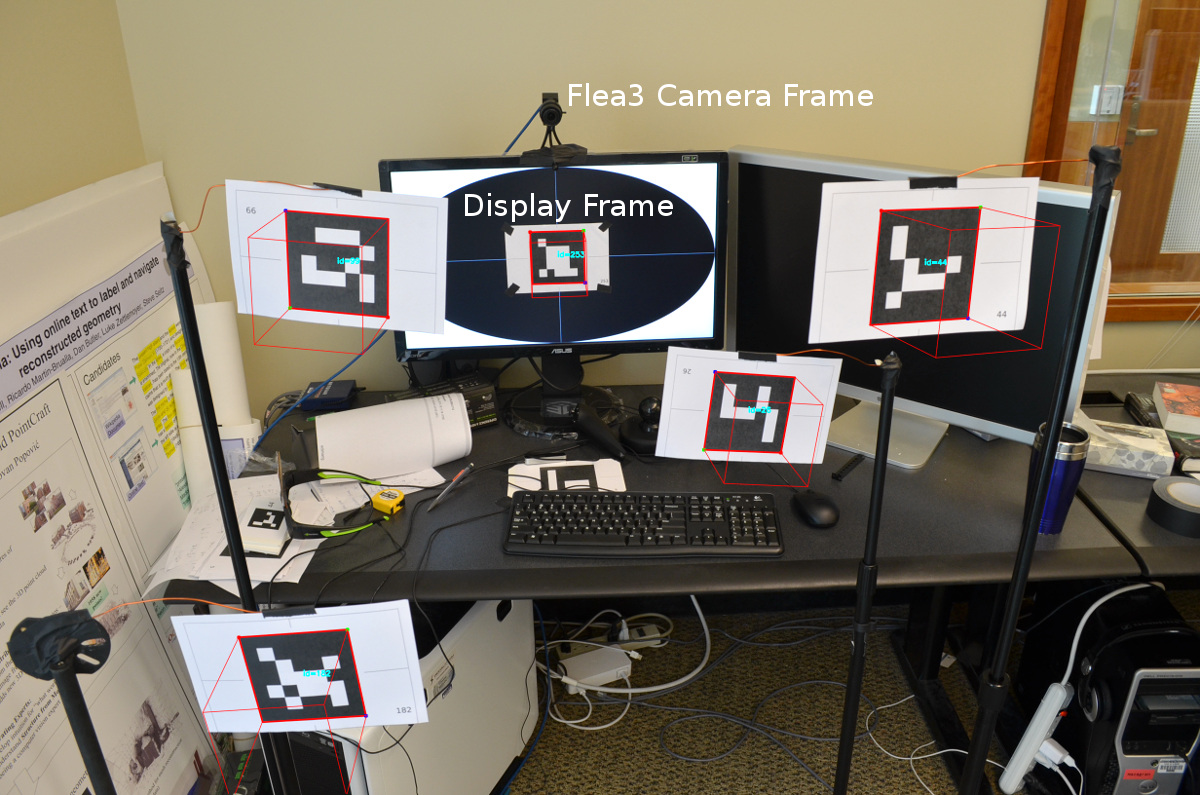
\includegraphics[width=\columnwidth]{calib1.jpg}
    \caption{Display - Camera registration setup}
    \label{fig:calib1}
\end{figure}

Registering the Leap input-frame with the display-frame follows a similiar process, see \figref{fig:calib2}.

\begin{figure}
    \centering
    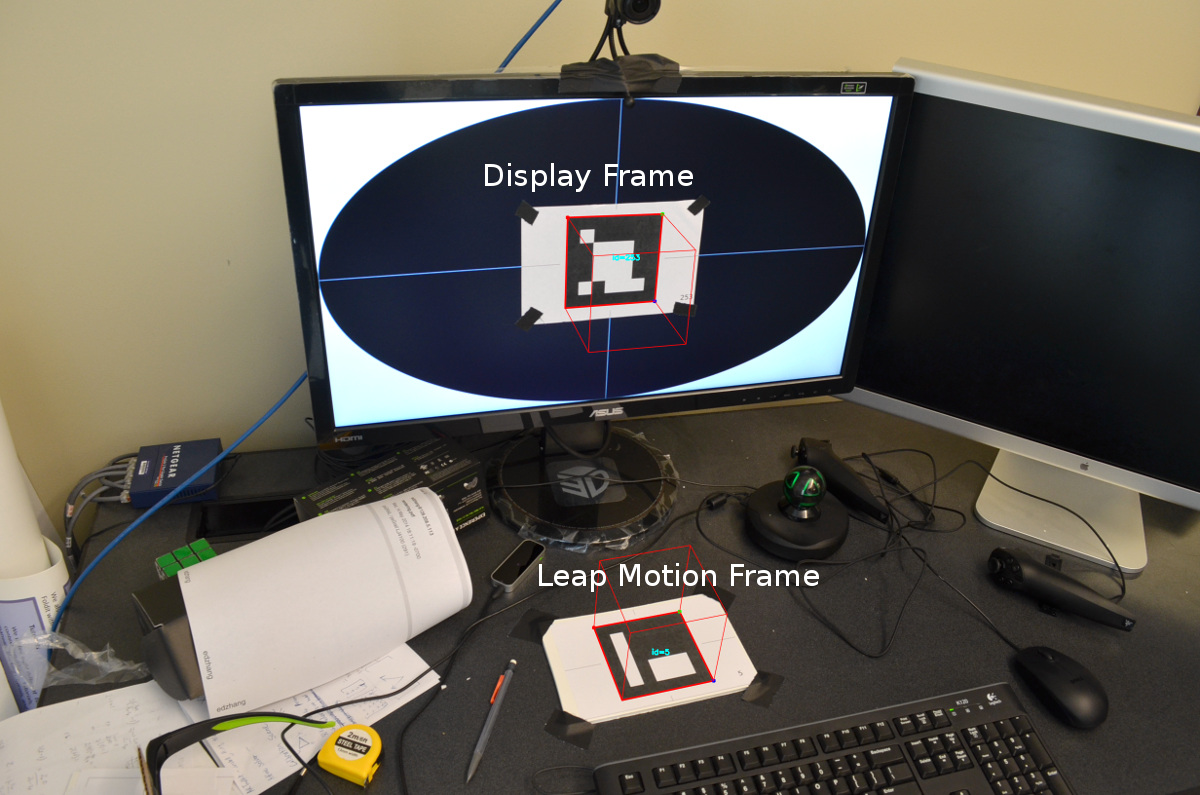
\includegraphics[width=\columnwidth]{calib2.jpg}
    \caption{Display - Input registration setup}
    \label{fig:calib2}
\end{figure}

As a result of this automatic calibration process, we were able to
successfully colocate coordinates in the Leap frame with the display-frame.
Because of limitations in the Leap hardware, such as nonlinearities in the
reported finger location, we implemented per-user tweaking functionality to
achieve adequate colocation over most the input space.
